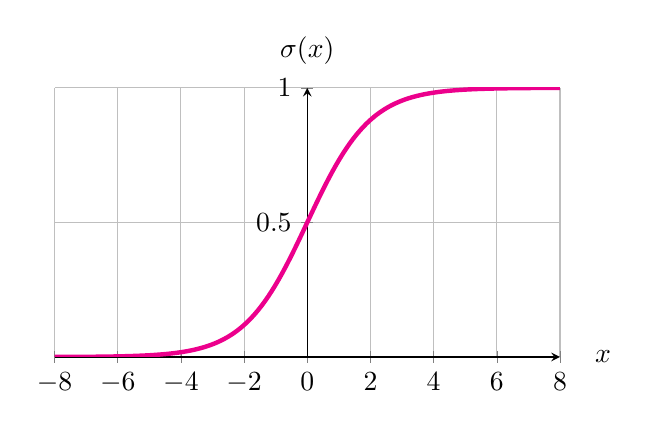
\begin{tikzpicture}
    \begin{axis}%
    [
        height=5cm,
        width=8cm,
        grid=major,     
        xmin=-8,
        xmax=8,
        axis x line=bottom,
        ytick={0,.5,1},
        ymax=1,
        axis y line=middle,
        xlabel=$x$,
        ylabel=$\sigma(x)$,
        every axis x label/.style={
            at={(ticklabel* cs:1.05)},
            anchor=west
        },
        every axis y label/.style={
            at={(ticklabel* cs:1.05)},
            anchor=south,
        },
    ]
        \addplot%
        [
            color=magenta,
            ultra thick,
            mark=none,
            samples=150,
            domain=-8:8,
        ]
        (x,{1/(1+exp(-x))});
    \end{axis}
\end{tikzpicture}